\chapter{Mendelian genetics (I)}

\section{Methodology and Results}
Mendel’s experiments were done using pea plants.
Contradictory to the notion that characteristics of an offspring are due to the blending of the parents’ traits, Mendel showed that the traits of the offspring do not appear in intermediate or blended traits. 

In his experiment with pea plants, he studied the patterns of inheritance in seven different features of the plant: flower color, flower position, stem length, seed shape, seed color, pod shape and pod color.
First, he established pea lines and grew them until they were purebred.
That is, the produced offspring are always identical to the parent.
He then performed cross-pollination experiments with the different variants of the pea and observed how traits were inherited.
He counted the number of offspring pea plants possessing each trait and found similar patterns for each of the seven features.

First, upon crossing peas with yellow seeds to those with green seeds, he observed that the first generation (F1) seeds were all yellow.
This shows that in the first generation after the cross, one form of a feature (dominant trait), such as yellow seed color, is visible and the other form (recessive trait), such as green seed color, is hidden. 

The F1 generation plants were then self-pollinated.
He observed that for the second generation, F2, the recessive trait reappeared in the minority of the offsprings.
That is, 3 out of 4 were yellow and 1 out of 4 was green.
He then thought that since the recessive trait (green) appeared in F2, the trait must have been present, although not expressed, in F1.

Mendel also analyzed purebred pea plants that differed in pairs of features, such as seed color (yellow and green) and seed shape (round and wrinkled).
He crossed yellow round seeds with green wrinkled seeds and observed that F1 seeds were all yellow and round - which shows that yellow and round are the dominant traits.
Then, upon self-pollination of the F1, he observed that the F2 generation plants were in the ratio $9:3:3:1$ ($\frac{9}{16}$ yellow round, $\frac{3}{16}$ yellow wrinkled, $\frac{3}{16}$ green round, and $\frac{1}{16}$ green wrinkled).
This is equivalent to 3 yellow to 1 green and 3 round to 1 wrinkled, which supports the idea that features are inherited independently.

\section{Synthesis}
With these patterns in mind, Mendel proposed that genes can be made controlled by pairs of heritable units (alleles) that came in different versions.
That is, genes are made by pairs of heredity units--AA, Aa, and aa where ‘A’ represents the dominant allele and ‘a’ represents the recessive allele.
He also theorized that an offspring inherits one unit of one trait from each parent.
This has been called the \emph{law of segregation}.
Following from the observation that there are independent features, a \emph{law of independent assortment} can be established.

Mendel's results can be summarized using a tool derived from the two laws described above, a Punnett square \cite{biomain}.
A Punnett square for one feature is in Figure \ref{fig:feat1}, while a Punnett square for two independent features is in Figure~\ref{fig:feat2}.

\begin{figure}[h]
    \centering
    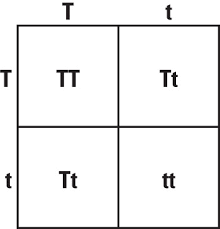
\includegraphics[scale=0.5]{feat1}
    \caption{Monohybrid cross Punnett square}
    \label{fig:feat1}
\end{figure}

\begin{figure}[h]
    \centering
    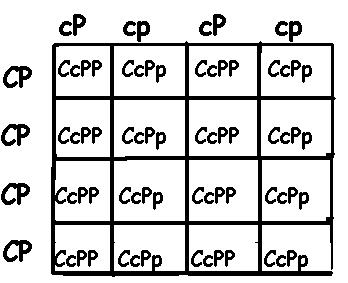
\includegraphics[scale=0.5]{feat2}
    \caption{Dihybrid cross Punnett square}
    \label{fig:feat2}
\end{figure}
